\documentclass[a4paper,12pt]{memoir}
\usepackage{cmap}
\usepackage[utf8]{inputenc}
\usepackage[russian]{babel}
\usepackage[TS1,T2A]{fontenc}
\usepackage{indentfirst}%делать отступ в начале параграфа 
\usepackage{amsmath,amssymb,amsfonts,amscd,amsthm}% расширенный набор матем. символов
\usepackage{bm}
\usepackage{color}% для использования цвета
\usepackage{graphicx} % для вставки рисунков
\usepackage{listingsutf8} % это лучше, чем verbatim
%\usepackage{russmath} % для корректного переноса матем. формул
\usepackage{hyperref}
\usepackage{pgf}

\long\def\title#1#2#3#4#5#6#7{
\mainmatter
\noindent
\thispagestyle{empty}

\vspace*{-\headheight}\vspace*{-\headsep}

\begin{center}
\textsc{ 
министерство образования и науки российской федерации\\
\textbf{\small{федеральное государственное автономное образовательное\\
учреждение высшего профессионального образования\\
<<Национальный исследовательский ядерный университет «МИФИ»}\\
(НИЯУ МИФИ)}\\
кафедра информационных систем и технологий\\
}

\vspace{4cm plus 1mm minus 1mm}


{\LARGE\textbf{КУРСОВАЯ РАБОТА}}

\vspace{1cm plus 1mm minus 1mm}

{\large
по дисциплине <<#1>>\\
на тему <<#2>>\\

\vfill

\begin{tabular}{l}
Группа\\
\\
Студент\\
\\
Руководитель работы\\
#5\\
\end{tabular}
\hfill
\begin{tabular}{l}
#3\\
\\
#4\\
\\
\\
#6\\
\end{tabular}

\vspace{3cm plus 1mm minus 1mm}

Москва #7
}

\newpage

% Обратная сторона титульного листа
\setcounter{page}{2}

\vspace*{1cm}
\section*{Аннотация}
\begin{quote} 
Работа посвящена модификации проектов «Компилятор формул»,
«Интерпретатор арифметических выражений» и«Выпуклая оболочка». В первом из этих проектов решалась задача расширения грамматики языка стекового компилятора определённой операцией, а также компиляции формул, содержащих эту операцию. Суть модификации второго проекта заключалась в вычислении значения выражений, содержащих операцию возведения в степень, которая считается левоассоциативной и имеющей минимальный приоритет. В проекте «Выпуклая оболочка» вычислялось расстояние от заданной прямой до выпуклой оболочки и максимальный радиус круга, содержащегося внутри выпуклой оболочки. В последнем из проектов вычилялась сумма рёбер, середина и оба из концов которых~--- <<хорошие>> точки, т.е. точки, проекция которых находится строго вне квадрата единичной площади с центром в начале координат и сторонами,  параллельными координатным осям.

\end{quote}

\tableofcontents*

\newpage

\end{center}

}

\def\+{\hskip 0.15mm}

\lccode`\-=`\-\defaulthyphenchar=127 %перенос слов с дефисами

\emergencystretch=2pt
\hfuzz=0.8pt

%Размер страницы
\settrimmedsize{297mm}{210mm}{*} % a4paper: 297mm * 210mm% 

% Оформление страницы
\pagestyle{plain}

%Размер текста
\settypeblocksize{46\baselineskip}{160mm}{*}
\setulmargins{*}{*}{1}
\setlrmargins{*}{*}{1}
\checkandfixthelayout
\typeoutlayout

\newcommand{\link}[1]{\texttt{#1}}

% Нумерация рисунков и таблиц сплошная по всему документу
\renewcommand{\thefigure}{\arabic{figure}}
\renewcommand{\theequation}{\arabic{equation}}
\addtodef{\mainmatter}{}{%
\counterwithout{figure}{section}%
\counterwithout{table}{section}%
%\counterwithout{longtable}{section}%
}

% Оформление секций
\makeatletter
\renewcommand*{\thesection}{\@arabic\c@section.}
\setsecnumformat{\csname the#1\endcsname\space}
\makeatother

\renewcommand{\thesubsection}{\large\arabic{subsection}}
%\setsecheadstyle{\centering\scshape}
\setbeforesecskip{\onelineskip}
\setaftersecskip{0.6\onelineskip}

%В подписях к рисункам разделитель - точка
%\captiondelim{ }
\captiondelim{.\space}
%Уменьшенный шрифт для подписей
\captionnamefont{\small\itshape}
\captiontitlefont{\small}
% Пробел до и после рисунка
\setlength{\intextsep}{6mm}
%\setlength{\textfloatsep}{3mm}
%Пробел до и после подписи к рисунку
\setlength{\abovecaptionskip}{2mm}
\setlength{\belowcaptionskip}{0mm}
\changecaptionwidth\captionwidth{0.85\linewidth}

%Убираем большие расстояния по вертикали в списках
\tightlists

% Оформление списка литературы
\setbiblabel{[#1]\hfill}
\renewcommand{\bibsection}{%
  \section*{Список литературы и интернет-ресурсов}
  \prebibhook}

\lstset{language=Ruby,inputencoding=utf8/koi8-r,basicstyle=\small,
stringstyle=\ttfamily,xleftmargin=1cm}

\begin{document}
\renewcommand{\contentsname}{{\Large{Содержание}\hfill}}

\title{Алгоритмы и структуры данных}
{Расширение языка стекового калькулятора операцией возведения в степень, которая является правоассоциативной и имеющей максимальный приоритет. Компилирование формул, содержащих данную операцию.
Вычисление значений выражений, содержащих операцию возведения в степень, которая считается левоассоциативной и имеющей минимальный приоритет. Вычисление расстояния от заданной прямой до выпуклой оболочки. Вычисление максимального радиуса круга, целиком содержащегося внутри выпуклой оболочки. Вычисление суммы длин рёбер полиэдра, середина и оба из концов которых~--- «хорошие» точки. }
{K04-361}
{Е.\+А.~Пономарёв}
{к.ф.-м.н., доцент}
{Е.\+А.~Роганов}
{2016}

\section{Введение}

В проектах «Компилятор формул» и «Интерпретатор арифметических
выражений» необходимо было расширить входную грамматику стекового компилятора операцией возведения в степень с указанными приоритетом и ассоциативностью, а также компилировать полученные формулы и вычислять соответствующие численные выражения. Реализация указанной модификации требует представления о формальных языках и грамматиках, об индуктивных функциях и простейших контейнерах данных. Так как в рамках учебного курса <<Алгоритмы и структуры данных>> проект должен быть реализован на языке Ruby, необходимы также базовые знания данного языка, как и знание основ объектно-ориентированного
программирования в целом~\cite{ruby}. 

Задачей проекта «Выпуклая оболочка»\cite{convex} является индуктивное 
перевычисление выпуклой оболочки последовательно поступающих точек плоскости и таких её
характеристик, как периметр и площадь. Целью данной работы является
определение расстояния от заданной прямой до выпуклой оболочки; вычисление радиуса максимального круга с центром в заданной точке, содержащегося в выпуклой оболочке. Решение этой задачи требует знания теории индуктивных функций, основ аналитической геометрии и векторной алгебры, а также языка Ruby~\cite{ruby}. Для наглядного изображения реализации задачи необходимы навыки работы с библиотекой графического интерфейса Tk~\cite{tk}. 

Проект «Изображение проекции полиэдра»~\cite{polyedr}~--- пример
классической задачи, для успешного решения которой необходимо знакомство с
основами вычислительной геометрии. Задачей, решаемой в данной работе, является
модификация эталонного проекта с целью определения суммы длин рёбер, середина и оба из концов которых~--- точки, проекция которых находится строго вне квадрата единичной площади с центром в начале координат и сторонами, параллельными координатным осям. Для этого необходимы хорошее понимание ряда разделов 
аналитической геометрии и векторной алгебры, основ объектно-ориентированного
программирования и языка Ruby. 


\section{Модификация проекта «Компилятор формул»}
\subsection*{Постановка задачи}
В проекте <<Компилятор формул>> была поставлена задача модифицировать эталонный проект следующим образом: <<В предположении, что язык стекового калькулятора расширен правоассоциативной и имеющей максимальный приоритет операцией \verb|^| возведения в степень, компилировать формулы, содержащие эту операцию>>.


С формальной точки зрения компилятор представляет собой программную реализацию некоторой функции: $\tau\colon L_1 \rightarrow L_2$,  действующей из множества цепочек одного языка $L_1$ в множество цепочек другого $L_2$ таким образом, что $\forall \omega \in L_1$  семантика цепочек $\omega$  и $\tau(\omega) \in L_2$  совпадает.
Нужный нам компилятор представляет собой программную реализацию отображения из множества цепочек языка $L(G_0)$  в множество цепочек языка $L(G_S)$ По этой причине его можно рассматривать, как функцию на пространстве последовательностей~\cite{stack}.

Рассмотрим в качестве входного языка $L(G_0)$ язык правильных арифметических формул, дополненный операцией  возведения в степень, являющейся правоассоциативной и имеющей максимальный приоритет. При этом грамматика $G_0$ вышеуказанного языка будет задаваться следующей НФБН:
\\

\begin{center}
\begin{tabular}{rll}
    $F  \rightarrow$ & $T$  &  $|$ $F+T$ $|$ $ \ F-T $\\
    $T  \rightarrow$ & $M$  &  $|$ $T*M$ $|$ $ \  T/M $\\
    $M  \rightarrow$ & $F$  &  $|$ $M$ \^~$F $   $|$ $ \ V $\\
    $V  \rightarrow$ & $a$  &  $| \ b  \ | \  c \  |  ...  |  \  z $\\ 
\end{tabular} 
\end{center}
Выходным языком будем считать язык $L(G_S)$ стекового калькулятора, грамматика $G_S$ которого также расширена указанной операцией  и задаётся такой НФБН:

\begin{center}
\begin{tabular}{rll}
     $e  \rightarrow \ e e + \ | \ e e - \ | \ e e * \ | \ e e / \ | \ e e$ \^~ $| \ a \ | \ b \ | \ ... \ | \ z \ $ \\
\end{tabular} 
\end{center}
\subsection*{Теоретические аспекты}

Стековый компилятор $\tau$ представляет собой программную реализацию отображения из множества цепочек языка $L(G_0)$ в множество цепочек языка $L(G_S)$. По этой причине его можно рассматривать, как функцию на пространстве последовательностей. Данная функция не является индуктивной, так как результатом компиляции двух произвольных цепочек $w_1 = a-b$ и $w_1 = (a-b)$ является одна и та же цепочка $a \ b \ -$. Если же дописать к обеим цепочкам $x=*c$, результаты компиляции соответствующих цепочек буду выглядеть следующим образом: $a \ b \ c \ * \ - \ $   и  $ \ a \ b \ - \ c \ *$. А это значит, что $\tau(w_1\circ x) \ne \tau(w_2\circ x)$.

Поэтому возникает необходимость построить индуктивное расширение $T$ функции $\tau$ для реализации однопроходного алгоритма. Очевидно, что рекурсивный компилятор формул не подходит для решения данной задачи, а значит, необходимо применить другой алгоритм, основанный на использовании тривиального стека. Для его реализации необходимо определить ряд условий: \\
\begin{itemize}
\item левая скобка \verb|(SYM_LEFT)| не предшествует ничему;
\item правая скобка \verb|(SYM_RIGHT)| предшествует всему;
\item одна арифметическая операция предшествует другой, если её приоритет не ниже, чем у второй;
\item если арифметическая операция является операцией возведения в степень~--- её приоритет выше, чем у какой-либо другой, и операции справа от неё выполняются согласно правилам правой ассоциативности.
\end{itemize} 


Для автоматической обработки конца формулы можно просто взять в скобки всю исходную формулу.

\subsection*{Описание используемых структур и применяемых алгоритмов}

Для решения задачи прежде всего необходимо реализовать тривиальный стек на базе вектора, чтобы размещать в нём отложенные операции. В языке Ruby массив (экземпляр класса Array) имеет все необходимые для этого методы, что только упрощает написание программного кода.
Также введём некоторые константы, задающие тип символа:
\begin{itemize}
\item \verb|SYM_LEFT = 0|  ~---  <<\verb|(|>> 
\item \verb|SYM_RIGHT = 1| ~--- <<\verb|)|>> 
\item \verb|SYM_OPER = 2| ~--- <<\verb|+|>>, <<\verb|-|>>, <<\verb|*|>>, <<\verb|/|>> 
\item \verb|SYM_OTHER = 3| ~---~ добавленная операция ~  \verb|^|
\end{itemize}


Модификация эталонного проекта заключается в повышении приоритета добавленной операции (возведения в степень) по отношению к другим операциям. Для этого в классе \verb|Compf| стекового компилятора, выведенного из уже реализованного класса \verb|Stack|, был изменён метод \verb|priority|:
\begin{lstlisting}
 def priority(c)
    return 3 if (c =='^') 

    (c == '+' or c == '-') ? 1 : 2
 end
\end{lstlisting}
Далее требуется изменить ассоциативность арифметической операции. Для этого необходимо в методе \verb|precedes?|, определяющем отношение предшествования, заменить \verb|>=| на \verb|>|:

\begin{lstlisting}
  def precedes?(a, b)
    return false if sym_type(a) == SYM_LEFT 
    return true  if sym_type(b) == SYM_RIGHT
    if (priority(a)==3 && priority(b)==3)
    priority(a) > priority(b) 
    else
    priority(a) >= priority(b)
    end
  end
\end{lstlisting}

 Многие значительно более сложные задачи на модификацию также сводятся к минимальным изменениям в тексте программы и не требует изменения структуры всей реализации в целом~\cite{stack}.

Ниже представлен снимок экрана, демонстрирующий работу программы: \\ \verb|compf.rb|:
\begin{figure}[ht!]
\begin{center}
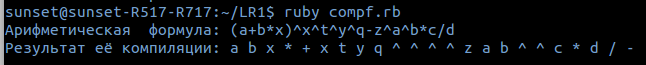
\includegraphics[width=1\hsize]{images/screen}
\end{center}
\caption{Вывод программы}\label{fig:screen}
\end{figure}



\section{Модификация проекта «Интерпретатор арифметических выражений»}
\subsection*{Постановка задачи}
В данном проекте задача была поставлена следующим образом: <<Вычисляются значения выражений, содержащих операцию возведения в степень, обозначаемую символом  \verb|^|, которая считается левоассоциативной и имеет минимальный приоритет>>.

Прежде всего, необходимо учесть, что в отличии от компилятора формул интерпретатор выражнений подразумевает наличие во входной формуле чисел (вместо идентификаторов переменных), а также необходимость выполнения получаемой выходной формулы (результата выражения) вместо её печати. По сути, к действиям, посредством которых был выполнен предыдущий проект, необходимо добавить класс \verb|Calc|, также выведенный из класса \verb|Stack|, и переопределить метод \verb|compile|, который будет вычислять значение входного арифметического выражения после работы соответствующего метода класса \verb|Compf|.

Рассмотрим в качестве входного языка $L(G_0)$ язык правильных арифметических формул, дополненный операцией возведения в степень, являющейся левоассоциативной и имеющей минимальный приоритет. При этом грамматика $G_0$ вышеуказанного языка будет задаваться следующей НФБН:
\\
\begin{center}

\begin{tabular}{rll}
    $F  \rightarrow$ & $T$  &  $| \ F+T \ $  $|$  $ \ F-T $\\
    $T  \rightarrow$ & $M$  &  $| \ T*M \ $  $|$  $ \ T/M $\\
    $M  \rightarrow$ & $F$  &  $| \ M$ \^~$F$ $|$  $ \ V $\\
    $V  \rightarrow$ & $0$  &  $| \ 1  \ | \  2 \  |  ... |  \  9 $\\
\end{tabular} \\
\end{center}
Грамматика $G_S$ выходного языка $L(G_S)$ задаётся такой НФБН: \\

\begin{center}
\begin{tabular}{rll}
	$e  \rightarrow \ e e \ | \ 0 \ | \ 1 \ | \ 2 \ | \ 3 \ | \ ... \ | \ 9 $ \\
\end{tabular}
\end{center}

\subsection*{Теоретические аспекты}
  Класс \verb|Calc| эталонного проекта был создан таким образом, чтобы добавлять новые числа в стек, а при появлении арифметической операции извлекать два числа из стека. Далее, после выполнения требуемого действия результат необходимо класть обратно в стек. При таком подходе, после завершения компиляции формулы, на вершине стекового калькулятора окажется результат вычисления арифметического выражения.
\subsection*{Описание используемых структур и применяемых алгоритмов}
 В данном случае суть модификации состояла в добавлении нового метода \\ \verb|involution|, определяющего операцию. Так как дополнительными условиями данной задачи являются минимальный приоритет и левоассоциативность операции, необходимо для правильной обработки случая, когда нам встречается данная операция, переопределить метод \verb|process_oper|:


\begin{lstlisting}

def involution(a,n)
  result =1
  if n>1
    n.times do
      result*=a
    end
  elsif n==1
    result=a
  elsif n==0
    result=1
  end
  return result
end

def process_oper(c)
    if c =='^'
      second,first = @s.pop,@s.pop
      @s.push(involution(first,second))
    else
    second, first = @s.pop, @s.pop
    @s.push(first.method(c).call(second))
    end
end
\end{lstlisting}

Ниже проиллюстрирован результат работы программы:
\begin{figure}[ht!]
\begin{center}
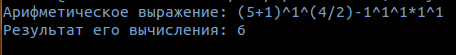
\includegraphics[width=0.8\hsize]{images/screen2}
\end{center}
\caption{Вывод программы}\label{fig:screen2}
\end{figure}

\section{Модификация проекта «Выпуклая оболочка»}
\subsection*{4.1 Постановка задачи}
В следующем проекте решалась задача вычисления расстояния от заданной прямой
до выпуклой оболочки. Кроме того, необходимо определять выпуклую оболочку и
 вычислять её характеристики сразу после поступления очередной точки. Для наглядного
  отображения работы программы необходимо графически иллюстрировать каждый этап,
   используя графический интерфейс Tk.

\subsection*{4.1 Теоретические аспекты}

 Пусть $X$~--- множество $\mathbb{R}^2$ точек плоскости,
  а $P$~--- совокупность всех выпуклых фигур на плоскости.
   Тогда тройка функций $f\colon X^* \rightarrow \mathcal{P}$ — выпуклая оболочка
    последовательности точек, $g\colon X^* \rightarrow \mathbb{R}$  — её периметр
     и  $h\colon X^* \rightarrow \mathbb{R}$ — её площадь, задаёт индуктивную
функцию $F\colon X^* \rightarrow \mathcal{P} \times \mathbb{R} \times \mathbb{R},$ $F = \begin{pmatrix}f\\ g\\ h\end{pmatrix}.$

 Пусть для некоторой последовательности точек плоскости выпуклая оболочка,
  а также её периметр и площадь, уже известны. Тогда после добавления
новой точки $x\in X$ возможны две ситуации: либо точка $x$ попадает внутрь оболочки,
 либо вне её.

Для получения новой оболочки необходимо, как это хорошо видно
 из следующего рисунка, удалить все освещённые рёбра, а концы оставшейся ломаной
  соединить двумя новыми рёбрами с добавляемой точкой $x$:
\begin{figure}[ht!]
\begin{center}
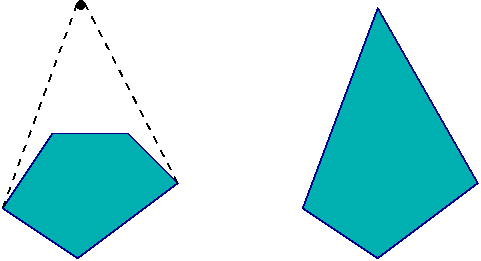
\includegraphics[width=0.4\hsize]{images/conv_2}
\end{center}
\caption{Удаление освещённых рёбер}\label{fig:conv_2}
\end{figure}

Если добавляемая точка лежит на продолжении одного из рёбер,
 то оболочка должна измениться, поэтому ребро, на продолжении которого лежит
  точка мы также будем считать освещённым:

\begin{figure}[ht!]
\begin{center}
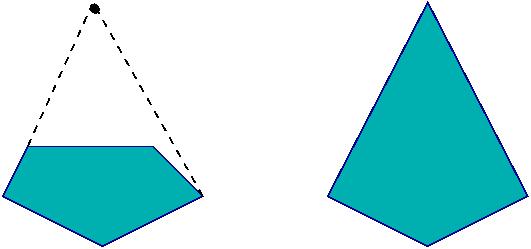
\includegraphics[width=0.4\hsize]{images/conv_3}
\end{center}
\caption{Удаление освещённых рёбер}\label{fig:conv_3}
\end{figure}

Для работы с точками на плоскости создаётся класс \verb|R2Point|. В нём необходим ряд
методов, которые позволяли бы вычислять \verb|расстояния| между точками,
сравнивать их на \verb|совпадение|, выяснять, лежат ли три точки на одной
прямой, находится ли некоторая точка на прямой \verb|между| двумя другими,
пересекаются ли отрезки, а также вычислять расстояние от заданной
прямой до выпуклой оболочки, сравнивая \verb|расстояние до отдельных рёбер|.
Кроме того, необходимо уметь вычислять \verb|площадь треугольника| и находить
все \verb|освещённые| ребра многоугольника.

Для вычисления площади треугольника в данном случае разумнее всего будет
воспользоваться векторным произведением $S = \frac{1}{2} |\vec a \times \vec b|$.
Тогда сократится количество необходимых вычислительных операций и результат будет более точным,
по сравнению с аналогичными способами вычисления.

Для векторов  $\vec a = (a_x, a_y, a_z)$ и $\vec b = (b_x, b_y, b_z)$  координаты вектора
 $\vec c$ находятся по формуле \\
\begin{center}
$\vec c = \left| \begin{array}{ccc} \vec i& \vec j& \vec k\\ a_x & a_y & a_z \\ b_x & b_y & b_z \end{array} \right| =$ $= (a_y b_z - a_z b_y) \vec i + (a_z b_x - a_x b_z) \vec j + (a_x b_y - a_y b_x) \vec k$.
\end{center}
Однако в том случае, когда векторы $\vec a$ и $\vec b$ расположены на плоскости,
их векторное произведение имеет единственную отличную от нуля компоненту,
вычисление которой и должно быть реализовано в методе \verb|area|.
Также важно то, что вычисляемая площадь является \verb|ориентированной|,
то есть может быть отрицательной.

Для вычисления расстояния от точки до прямой используется метод \verb|dist_to_line|.
 В его основу положена хорошо известная формула:

 $$d = \frac{|A\times M_x+B\times M_y+C|}{\sqrt{A^2+B^2}}$$. Коэффициенты  \verb|A|, \verb|B| и \verb|C|
 мы получаем из общего вида уравнения прямой, проходящей через две точки:
   $ \left(y_1-y_2\right)x+\left(x_2-x_1\right)y+\left(x_1y_2-x_2y_1\right)=0. $

Ниже приведена реализация метода \verb|dist_to_line|:

\begin{lstlisting}
 def dist_to_line(m,n)
    a = (n.y-m.y)
    b = (m.x-n.x)
    c = m.x*(m.y-n.y)+m.y*(n.x-m.x)
    ((a*@x+b*@y+c).abs/Math.sqrt(a*a+b*b))
 end
\end{lstlisting}


\subsection*{4.1 Описание используемых структур и применяемых алгоритмов}

Определение того факта, лежат ли три точки на одной прямой (это делает
метод \verb|triangle?|), сводится к вычислению площади треугольника
и сравнению её с нулём; а для того, чтобы точка $T$ прямой находилась на отрезке
$[A,B]$ этой же прямой (проверяет справедливость этого факта
метод экземпляра \verb|inside?|), необходимо и достаточно принадлежности
проекций этой точки проекциям на оси координат отрезка $[A,B]$.

Для того чтобы реализовать метод \verb|light?|, позволяющий выяснить,
освещено ли ребро $[A,B]$ выпуклой оболочки из данной точки, дадим строгое определение освещённости.
Ребро [A,B] называется освещённым из точки $T$, если ориентированная
площадь треугольника, образованного точками $A, B$ и $T$ отрицательна, либо если
точка $T$ расположена на прямой, проходящей через точки $A$ и $B$ вне отрезка [A,B].

Искомое расстояние от заданной прямой до выпуклой оболочки будет отлично от нуля
в том случае, если прямая не пересекает ни одно ребро данного многоугольника.
Метод \verb|intersect?| будет вычислять взаимное расположение
отрезков, заданных точками класса \verb|R2Point|, при помощи векторных произведений.

Пусть даны два отрезка. Первый задан точками $P_1(x_1;y_1)$ и $P_2(x_2;y_2)$.
 Второй задан точками $P_3(x_3;y_3)$ и  $P_4(x_4;y_4)$.

\begin{figure}[ht!]
\begin{center}
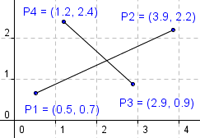
\includegraphics[width=0.4\hsize]{images/conv_4}
\end{center}
\caption{Взаимное расположение отрезков}\label{fig:conv_4}
\end{figure}

\newpage
Тогда их взаимное расположение проверяется с помощью векторных произведений
 (каждое из них реализуется методом \verb|cross|):
\begin{center}
$v_1 = |\vec {P_3P_4} \times \vec {P_3P_1}|, $
$v_2 = |\vec {P_3P_4} \times \vec {P_3P_2}|$

$v_3 = |\vec {P_1P_2} \times \vec {P_1P_3}|, $
$v_4 = |\vec {P_1P_2} \times \vec {P_1P_4}|$.
\end{center}
Рассмотрим отрезок $P_3P_4$ и точки $P_1$ и $P_2$.

\begin{figure}[ht!]
\begin{center}
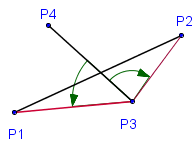
\includegraphics[width=0.5\hsize]{images/conv_5}
\end{center}
\caption{}\label{fig:conv_5}
\end{figure}

Точка $P_1$ лежит слева от прямой $P_3P_4$. Для неё
векторное произведение

 $v_1 = |\vec {P_3P_4} \times \vec {P_3P_1}| > 0,$
так как векторы положительно ориентированы.
Точка $P_2$ расположена справа от прямой $P_3P_4$. Для неё
 векторное произведение

 $v_2 = |\vec {P_3P_4} \times \vec {P_3P_2}| < 0,$
 так как векторы отрицательно ориентированы.

Для того чтобы точки $P_1$ и $P_2$ лежали по разные стороны от прямой $P_3P_4$,
 достаточно, чтобы выполнялось условие $v_1v_2 < 0$ (векторные произведения имели противоположные  знаки).

Аналогичные рассуждения можно провести для отрезка $P_1P_2$ и точек $P_3$ и $P_4$.

Итак, если $v_2 = |\vec {P_3P_4} \times \vec {P_3P_2}| < 0,$ то отрезки пересекаются.

Ниже представлена реализация указанных методов:

\begin{lstlisting}

 def cross(w)
    @x*w.y-w.x*@y
 end

 def R2Point.intersect?(a,b,c,d)
    h = R2Point.new((d.x-c.x),(d.y-c.y))
    j = R2Point.new((a.x-c.x),(a.y-c.y))
    k = R2Point.new((b.x-c.x),(b.y-c.y))
    return true if h.cross(j)*h.cross(k) < 0
    false
 end
\end{lstlisting}


Далее необходимо определить контейнер для хранения точек выпуклой оболочки.
 Наиболее подходящим в данном случае является дек, так как его можно свернуть
  в кольцо и считать <<текущим>> то ребро оболочки, которое соединяет начало и конец дека.
   Дальнейшие операции проводятся применительно к этому ребру:

\begin{figure}[ht!]
\begin{center}
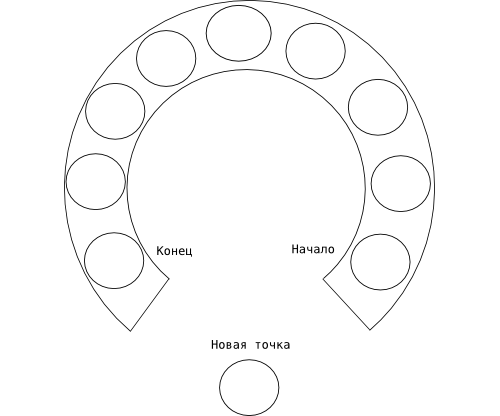
\includegraphics[width=0.6\hsize]{images/conv_6}
\end{center}
\caption{Дек, содержащий точки}\label{fig:conv_6}
\end{figure}
 Для того чтобы удалить все освещенные ребра необходимо, <<повернуть>> дек таким образом,
  чтобы концы одного из освещённых рёбер находились в конце и в начале дека соответственно
  (если только освещённые рёбра вообще существуют). После этого нужно удалить найденное ребро.


Проектирование основных классов выполнено следующим образом:
 cоздаётся базовый класс \verb|Figure| (фигура), и из него выводятся необходимые
  нам классы: \verb|Void| (нульугольник), \verb|Point| (одноугольник),
   \verb|Segment| (двуугольник) и \verb|Polygon| (многоугольник).

\begin{figure}[ht!]
\begin{center}
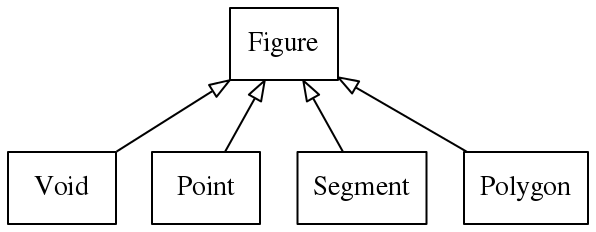
\includegraphics[width=0.7\hsize]{images/conv_7}
\end{center}
\caption{Иерархия классов}\label{fig:conv_7}
\end{figure}

Каждый из последних четырёх классов должен реализовывать методы \verb|add| (добавить новую точку),
\verb|perimeter| (получить периметр выпуклой оболочки) и \verb|area| (получить площадь выпуклой оболочки).
 При этом объект типа \verb|Point| должен содержать внутри себя одну точку (компоненту
  типа \verb|R2Point|), объект типа \verb|Segment|~--- две, а типа \verb|Polygon|~--- целый дек точек.

Вернемся к цели данной модификации, а именно~--- вычислению расстояния
 от заданной прямой до выпуклой оболочки. Прежде всего, мы будем хранить 2 точки,
  задающие прямую, как экземпляры класса \verb|Figure|: @@apoint, @@bpoint.
   Нужный параметр @@d(расстояние) следует переопределять для каждой фигуры,
    начиная с одноугольника. Ниже приведен листинг, демонстрирующий модификацию конкретных
     классов программы.
Для \verb|Segment|:
\begin{lstlisting}
def initialize(p, q)
  @p, @q = p, q
  @@intersect = R2Point.intersect?(@p,@q,@@apoint,@@bpoint)
  @@d = 0.0 if @@intersect
  if @q.dist_to_line(@@apoint,@@bpoint)<@@d && !@@intersect
    @@d = @q.dist_to_line(@@apoint,@@bpoint)
  end
...
end
\end{lstlisting}

Для \verb|Polygon|:
\begin{lstlisting}
...
if c.dist_to_line(@@apoint,@@bpoint)<@@d && !@@intersect
@@d = c.dist_to_line(@@apoint,@@bpoint)
end
...
\end{lstlisting}

При этом, в случае добавления двух новых рёбер в дек искомое расстояние изменится,
 а следовательно, его необходимо перевычислить. В случае пересечения прямой и
 выпуклой оболочки расстояние необходимо приравнять к нулю.
\begin{lstlisting}
...
@intersect=R2Point.intersect?(t,@points.first,@@apoint,@@bpoint)

if !@@intersect
 @@intersect=R2Point.intersect?(t,@points.last,@@apoint,@@bpoint)
end

@@d = 0.0 if @@intersect

if t.dist_to_line(@@apoint,@@bpoint)<@@d && !@@intersect
  @@d = t.dist_to_line(@@aline,@@bline)
end

@points.push_first(t)
...
\end{lstlisting}


\subsection*{4.2 Постановка задачи}
В следующем проекте решалась задача вычисления радиуса максимального круга с
центром в заданной точке, содержащегося в выпуклой оболочке. Кроме того, необходимо
определять выпуклую оболочку и вычислять её характеристики сразу
после поступления очередной точки.
Для наглядного отображения работы программы необходимо
графически иллюстрировать каждый этап, используя графический интерфейс Tk.
\subsection*{4.2 Теоретические аспекты}

Помимо вышеописанных методов и алгоритмов, используемых в выполнении
 предыдущей модификации, необходимо индуктивно
 вычислять максимальный радиус вписанной окружности, т.е. минимальное из  расстояний
  от заданного центра до каждого из рёбер выпуклой оболочки.


\subsection*{4.2 Описание используемых структур и применяемых алгоритмов}\
В общем случае необходимо искать минимальное из расстояний
от заданного центра до каждого ребра выпуклой оболочки (если центр лежит внутри многоугольника).
Если же центр окружности находится вне оболочки~--- радиус вписанной окружности будет равен нулю.



 В первую очередь, необходимо  объявить экземпляр класса \verb|Figure| для центра окружности,
  и метод, который будет вычислять искомый радиус:
\begin{lstlisting}
@@center = nil
def radius; @@R end
\end{lstlisting}

Далее, при первом же вычислении радиуса многоугольника необходимо проверить, лежит ли центр
 внутри выпуклой оболочки:

\begin{lstlisting}
def outside?
   @points.size.times do
     break if @@center.light?(@points.last, @points.first)
     @points.push_last(@points.pop_first)
   end
   @@center.light?(@points.last, @points.first)
end
\end{lstlisting}

Для общего случая будем сразу выполнять эту проверку и в случае надобности   обнулять переменную  @@R, отвечающую за радиус:
\begin{lstlisting}
  outside?() ?  @@R = 0 :  @@R = [@@center.dist_to_line(a,b),
  @@center.dist_to_line(b,c),@@center.dist_to_line(a,c)].min

\end{lstlisting}

Ниже приведён графический вывод работы программы для заданных точек:
\begin{figure}[ht!]
\begin{center}
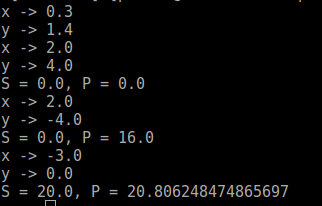
\includegraphics[width=0.5\hsize]{images/poly}
\end{center}
\caption{Ввод данных}\label{fig:poly}
\end{figure}

\begin{figure}[ht!]
\begin{center}
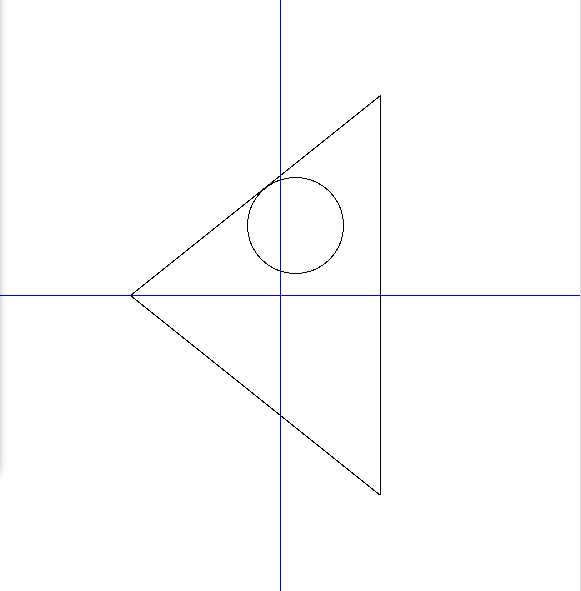
\includegraphics[width=0.5\hsize]{images/poly1}
\end{center}
\caption{Вывод в Tk}\label{fig:poly1}
\end{figure}


 В приложении приведены  реализации некоторых технических моментов, связанных с изменением выпуклой оболочки.



\section{Модификация проекта <<Изображение проекции полиэдра>>}
\subsection*{Постановка задачи}

Пусть точку в пространстве назывется <<хорошей>>, если её проекция находится строго вне квадрата единичной площади с центром в начале координат и сторонами, параллельными координатным осям.   
В данном прокте необходимо было модифицировать эталонный проект таким образом, чтобы определялась и печаталась следующая характеристика полиэдра: сумма длин рёбер, середина и оба из концов которых~--- <<хорошие>> точки.

В общем случае, для успешного решения задачи необходимо знакомство с основами вычислительной геометрии.

\subsection*{Теоретические аспекты}

Для начала приведём некоторые понятия.


\verb|Полиэдр (polyedr)|~--- Множество выпуклых плоских многоугольников. 

\verb|Грань полиэдра (facet)|~--- Выпуклый плоский многоугольник. 

\verb|Ребро полиэдра (edge)|~--- Любая из сторон одной из граней. 

\verb|Вершина полиэдра (vertex)|~--- Любая из вершин произвольной грани. 


\begin{figure}[ht!]
\begin{center}
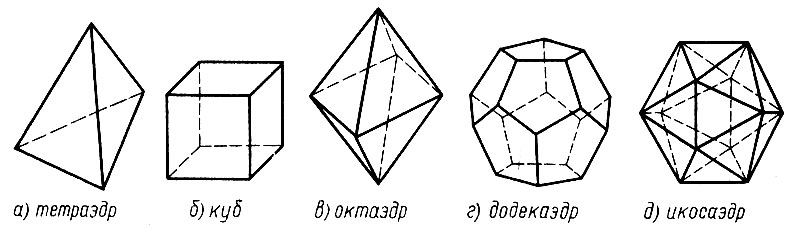
\includegraphics[width=0.9\hsize]{images/poly2}
\end{center}
\caption{Некоторые виды полиэдров}\label{fig:poly2}
\end{figure}


В рассматриваемом проекте речь идёт о геометрических объектах, находящихся в трёхмерном пространстве, поэтому необходимо вспомнить некоторые факты из линейной алгебры и аналитической геометрии.

Прежде всего вследует вспомнить, что точку пространства $\mathbb R^3$ можно задать с помощью трёх действительных чисел~---  её координат. Эти же координаты задают и вектор трёхмерного пространства, начало которого совпадает с началом координат, а конец~---  с рассматриваемой точкой.

Для векторов в пространстве определены операции сложения, вычитания и умножения на число, порождающие новый вектор, координаты которого находятся с помощью сложения, вычитания и умножения на число координат исходных векторов.

Также необходимо знание  скалярного, векторного и смешанного произведения векторов, и уметь использовать данные операции.

 Помимо прочего, в данном проекте необходимо использовать линейные преобразования (отображения) плоскости и пространства. Любое такое преобразование, как известно, задаётся квадратной матрицей порядка два для плоскости и порядка три для пространства. Напомним, что тождественному преобразованию соответствует единичная матрица $E$.

Среди всех преобразований в данном случае особенно интересны повороты и гомотетия, задаваемая матрицей вида $kE,$ где $k$~---  положительная константа, а $E$~---  единичная матрица.  
Ортогональные преобразования плоскости и пространства, сохраняющие ориентацию, являются поворотами. На плоскости поворот на угол $\varphi$ задаётся матрицей вида

\begin{center}
$\begin{pmatrix}\cos\varphi&\sin\varphi\\ -\sin\varphi&\cos\varphi\end{pmatrix}.$
\end{center}.

В случае пространства повороту на угол $\varphi$ вокруг оси $Oz$ соответствует следующая матрица: 
\begin{center}
$\begin{pmatrix}\cos\varphi& \sin\varphi & 0 \\ -\sin\varphi&\cos\varphi& 0\\
0 & 0 & 1\end{pmatrix}.$
\end{center}.

Аналогичный вид имеют и матрицы поворота вокруг осей $Ox$ и $Oy,$ а произвольное вращение пространства может быть представлено в виде композиции трёх последовательных поворотов вокруг осей $Oz, Oy$ и вновь $Oz$.

В процессе работы над проектом нам потребуется решать следующую задачу: найти пересечение отрезка с полупространством, которое задано точкой на граничной плоскости и вектором внешней нормали к ней. Двумерный аналог этой задачи таков: найти пересечение отрезка на плоскости с полуплоскостью, которая задана точкой на граничной прямой и вектором внешней нормали к этой прямой. Рассмотрим решение последней из задач.

Пусть концы отрезка $B$ (от английского слова \verb|begin|) и $F$ (от \verb|final|) имеют соответственно координаты $(x_1, y_1)$ и $(x_2, y_2)$ точка на граничной прямой~---  координаты $(x_0, y_0),$ а вектор внешней нормали к полуплоскости~---  это вектор $\overrightarrow N$.

Для этого необходимо и достаточно, чтобы оба конца отрезка лежали с «нужной» стороны от заданной прямой.

Точка $(x_1, y_1)$ будет лежать с <<нужной>> (внешней по отношению к полуплоскости) стороны от граничной прямой, если угол между векторами внешней нормали и вектором, соединяющим точки $(x_0, y_0)$ и $(x_1, y_1)$ является острым.

Искомое условие имеет следующий вид: $\overrightarrow N \cdot \overrightarrow{AB} > 0.$
Тогда для того чтобы пересечение отрезка с полуплоскостью представляло собой пустое множество, необходимо чтобы:
$\overrightarrow N \cdot\overrightarrow{AB} > 0 \wedge \overrightarrow N \cdot \overrightarrow{AF} > 0$.

Если знаки указанных скалярных произведений разные, то отрезок пересекает прямую, ограничивающую полуплоскость. В этом случае для определения пересечения отрезка с полуплоскостью прежде всего необходимо найти точку их пересечения. Произвольная точка отрезка $BF$ может быть записана как $(1-t)B + tF,$ где $0 \leqslant t \leqslant 1$. При $t = 0$ эта формула задаёт начало отрезка (точку $B$ ), а при $t=1$~---  его конец (точку $F$). Отсюда следует, что искомая точка пересечения в свою очередь соответствует значению  $$t = \frac{\overrightarrow N \cdot \overrightarrow{AB}} {\overrightarrow N \cdot \overrightarrow{AF} - \overrightarrow N \cdot \overrightarrow{AB}},$$ так как для неё $\overrightarrow N \cdot \overrightarrow{AC} = 0$.
 
\subsection*{ Описание используемых структур и применяемых алгоритмов}

Точку в трёхмерном пространстве ($\mathbb R^3$), так же, как и вектор этого пространства, мы будем представлять объектом класса \verb|R3|, имеющем три действительные компоненты (\verb|@x, @y| и \verb|@z|),~---  координаты точки или вектора. В этом классе реализуем ряд методов, обеспечивающих все необходимые в данном проекте манипуляции над точками  (векторами).

Каждое из рёбер (экземпляров класса \verb|Edge|) полиэдра будем задавать его началом и концом~---  объектами класса \verb|R3|, а произвольную его грань (экземпляр класса \verb|Facet|)~---  массивом её вершин. Сам полиэдр будет являться экземпляром класса \verb|Polyedr|, в конструкторе (методе \verb|initialize|) которого будет обрабатываться файл, содержащий всю информацию о полиэдре.

Так как плоскость проектирования горизонтальна, то достаточно <<забыть>> $z$-координату.

Теперь рассмотрим некоторые программистские аспекты. Модификация данного проекта довольна проста и, по сути, заключается в добавлении нового параметра~---  суммы длин рёбер, середина и оба из концов которых~---  «хорошие» точки. Следовательно  вся задача сводится к определению <<хороших>> точек ребра и  умению вычислять середину отрезка.

Найдем обратное условие, когда данная нам точка не является  <<хорошей>>. Очевидно, что оно будет выглядеть  следующим образом (так как мы рассматриваем проекцию ~---  нет смысла включать в условие координату  \verb|z|):
\begin{center}
 $x,y < 0.5$ & $x,y > -0.5$
\end{center}

 
Учитывая коэффициент гомотетии и данное условие, можно написать необходимый метод:
\begin{lstlisting}
def good?(c)
   return false if ((@x.abs<0.5*c)&&(@y.abs<0.5*c))
   true
end
\end{lstlisting}

Середина отрезка находится стандартным способом:

Пусть заданы два конца отрезка в пространстве $A(x_a,y_a,z_a)$ и $B(x_b,y_b,z_b),$ тогда середина отрезка имеет следующие координаты:

 $$x_c = \frac {x_a+x_b}2, \ y_c = \frac {y_a+y_b}2, \ z_c = \frac {z_a+z_b}2.$$
 

Для реализации данного метода у класса  \verb|Edge|(Ребро) есть две переменные  \verb|@@beg|, \verb|@@fin|, отвечающие за начало и конец отрезка.  Учитывая то, что каждая из этих точек уже имеет свои координаты, метод нахождения середины отрезка будет выглядеть следующим образом:  

\begin{lstlisting}
def middle
   (@beg+@fin)/2
end
\end{lstlisting}

Исходя из всего вышеупомянутого, можно написать метод вычисления длины ребра. Чтобы найти длину отрезка можно воспользоваться скалярным произведением векторов. Для этого необходимо ребро превратить в вектор, то есть взять разность \verb|@fin-@beg|, обозначить её как  $\vec A,$  и используя метод класса  \verb|R3 dot|, вычислить квадратный  корень из скалярного квадрата вектора  $\vec A$.  Ниже представлена реализация методов \verb|dot|  и \verb|length|.
\begin{lstlisting}
def dot(other) 
   @x*other.x+@y*other.y+@z*other.z
end
\end{lstlisting}


\begin{lstlisting}
def length(c)
   if (@beg.good?(c) && @fin.good?(c) && self.middle)
     a=(@fin-@beg)*(1/c)
     Math.sqrt(a.dot(a))
   else
     0
   end
end 
\end{lstlisting}


Итак, всё что остаётся сделать~--- при задании нового ребра его вершинами, проверять координаты начала, конца и середины ребра на <<хорошие>> точки, и суммировать подходящие нам рёбра. Всё это реализуется в классе \verb|Polyedr|,  в цикле задания рёбер очередной грани:


\begin{lstlisting}
(0...size).each do|n| 
     e = Edge.new(vertexes[n-1],vertexes[n])
     @edges << e
     @length += e.dist(c)
end
\end{lstlisting}




\newpage
\begin{thebibliography}{}

\bibitem{ruby}
\link{http://ru.wikipedia.org/wiki/Ruby}~---
Википедия (свободная энциклопедия) о языке Ruby.

\bibitem{convex}
\link{https://home.mephi.ru/files/2373/material\_ici\_toc.zip/index.html}~---
Описание проекта «Выпуклая оболочка».

\bibitem{tk}
\link{http://www.tkdocs.com/tutorial/install.html}~---
Описание проекта «Выпуклая оболочка».


\bibitem{polyedr}
\link{https://home.mephi.ru/files/3214/material\_ici\_toc.zip/index.html}~---
Описание проекта «Изображение проекции полиэдра».

\bibitem{stack}
\link{https://home.mephi.ru/files/2077/material\_ici\_toc.zip/index.html}~---
Описание проекта Стековый компилятор формул.


\end{thebibliography}

\newpage
\section{Приложение к пункту 4.2}

В участки кода программы, отвечающие за удаление освещённых рёбер и добавление новых, были внесены следующие изменения:

При удалении или добавлении рёбер с некоторой вероятностью придётся пересчитывать радиус
  вписанной окружности. На самом этапе удаления ему будет временно присваиваться значение
    \verb|-1.0|. Далее искомый радиус будет вычисляться в зависимости от ситуации.


Учёт удаления ребра, соединяющего конец и начало дека:
\begin{lstlisting}
if (@@R - @@center.dist_to_line(@points.last,@points.first))<EPS
   @@R = -1.0
end
\end{lstlisting}


 Удаление освещённых рёбер из начала дека:
\begin{lstlisting}
@@R = -1.0 if @@R == @@center.dist_to_line(p, @points.first)
\end{lstlisting}

Удаление освещённых рёбер из конца дека:
\begin{lstlisting}
@@R = -1.0 if @@R == @@center.dist_to_line(p, @points.last)
\end{lstlisting}

В случае, если надо переопределить радиус вписанной окружности, мы также ищем минимальное
 из расстояний от центра до каждого ребра.

\begin{lstlisting}
if @@R == -1.0
  @@R = @@center.dist_to_line(@points.last, @points.first)
  @points.size.times do
    if @@R > @@center.dist_to_line(@points.last, @points.first)
    end
    @@R = @@center.dist_to_line(@points.last, @points.first)
    @points.push_last(@points.pop_first)
  end
else
 @@R=[@@R,@@center.dist_to_line(@points.last, @points.first)].min
 @points.push_last(@points.pop_first)
 @@R=[@@R,@@center.dist_to_line(@points.last, @points.first)].min
end
\end{lstlisting}



\end{document}
